\subsection{Human Protein Atlas membrane annotation: surface exposure of gated antigens}
\label{sec:hpa}
CAR--T accessibility requires that a gated antigen be physically exposed at
the plasma membrane. We audited Human Protein Atlas (HPA) per-gene records
(per-gene TSV endpoint, one accession-level record per Ensembl gene) for all
@NGENES@ genes in the study universe; @NOK@ genes had an HPA record and
@NNOREC@ had none (@NORECLIST@, both pseudogenes). Two annotation tiers were
scored: the sequence-based HPA protein-class call (\emph{Predicted membrane
proteins}) and the antibody-based immunofluorescence (IF) subcellular
location.

\paragraph{Calibration gate.} For the protein-class tier we required (G1) at
least 3/4 approved references (CD19, ERBB2, FOLR1, TNFRSF17)
predicted-membrane (observed @GATEONE@), (G2) 0/4 intracellular controls
(POLR2A, RPS3, PCNA, PSMA1) predicted-membrane (observed @GATETWO@), and
(G4) 0/4 controls with IF plasma membrane (observed @GATEFOUR@); this gate
PASSED. The pre-registered IF gate G3 ($\geq$2/4 references with IF plasma
membrane) FAILED by construction: only 2/4 references have any HPA IF
subcellular record at all (CD19 - the most clinically validated CAR antigen
- and FOLR1 are uncovered), leaving a denominator of two. We record the
first-pass failure and apply a revised non-contradiction gate G3r ($\geq$1
covered reference with IF plasma membrane; observed @GATETHREE@, passed by
ERBB2), using the IF tier descriptively per antigen with no group-level IF
claims.

\paragraph{Membrane prediction does not enrich the gated set (null).}
@GATEDPM@ of gated genes versus @BGPM@ of background genes are predicted
membrane proteins (Fisher odds ratio @FISHEROR@, $p=@FISHERP@$).
Topology-stratified control is degenerate here: within every annotated
membrane-topology stratum (single-pass, multi-pass, GPI) essentially all
genes of both groups are predicted membrane, leaving only the unannotated
stratum informative, so the Cochran--Mantel--Haenszel estimator reduces to
that single stratum (@CMHOR@, $p=@CMHP@$). HPA membrane prediction largely
restates UniProt topology and carries no additional signal distinguishing
the gated set.

\paragraph{The experimental IF tier is sparse and study-biased.} Only
@IFCOVG@ of gated and @IFCOVB@ of background genes have any IF subcellular
record; the coverage difference is itself significant (Fisher odds ratio
@IFCOVOR@, $p=@IFCOVP@$), i.e.\ IF profiling preferentially covers the
better-studied gated/cancer genes, so IF absence is not evidence of
non-surface localization. Per-antigen calls (Table~\ref{tab:hpa}) are
nonetheless actionable: CA9, MSLN and PSCA carry \emph{Supported} IF
plasma-membrane main locations, and CLDN18 is called \emph{Cell Junctions}
(Approved) - the biologically correct surface compartment for a
tight-junction claudin. SLC39A6 is the weakest antigen: its only IF record
is \emph{Uncertain} with main location Cytosol, compounding its heaviest
glycan shield in Section~\ref{sec:glygen}; on two orthogonal axes it is the
least validated AND-gate antigen. CA12 and CLDN6 have no IF record at all.

\begin{table}[t]
\centering\small
\caption{HPA membrane annotation for AND-gate antigens and approved
references. PM = plasma membrane; IF main = HPA IF main location (blank = no
IF record).}
\label{tab:hpa}
\begin{tabular}{lllll}
\hline
gene & role & predicted membrane & IF PM & IF main location \\
\hline
@ANTIGENROWS@
\hline
\end{tabular}
\end{table}

\begin{figure}[t]
\centering
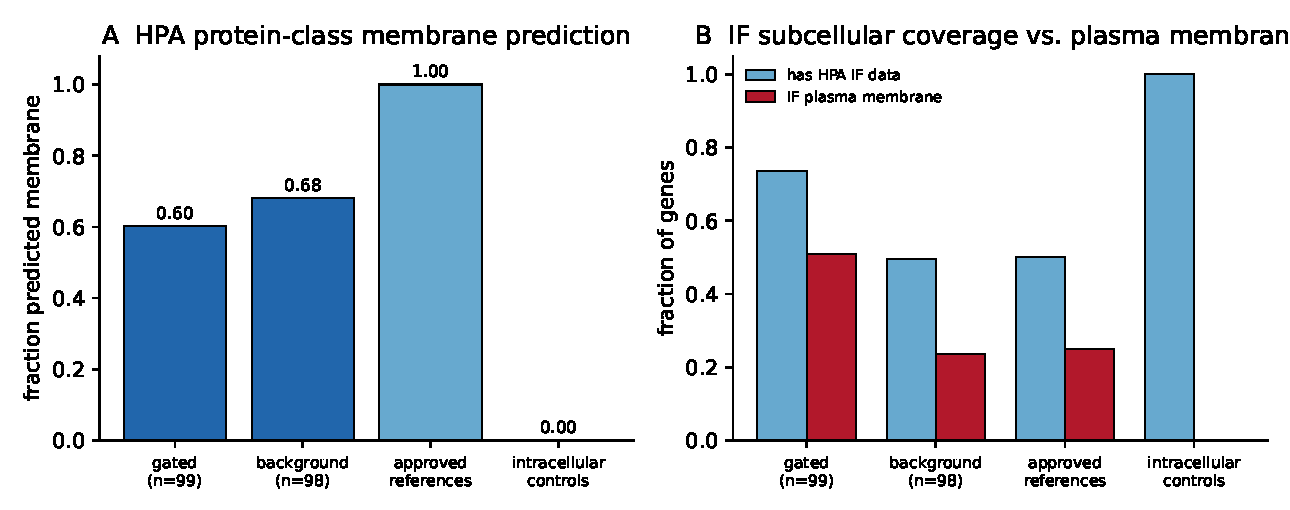
\includegraphics[width=\textwidth]{hpa_fig.pdf}
\caption{HPA membrane annotation by gene group. (A) Fraction predicted
membrane proteins; the gated set is not enriched over background. (B) IF
subcellular coverage versus IF plasma-membrane calls; the experimental tier
covers only a minority of genes and preferentially the gated ones.}
\label{fig:hpa}
\end{figure}
